\documentclass[runningheads]{llncs}

\usepackage[T1]{fontenc}
\usepackage{graphicx}
\usepackage{subcaption}
\usepackage{float}
\usepackage{amsmath}
\usepackage{hyperref}
\usepackage{cite}
\usepackage{url}

\begin{document}

\title{Pitch control: A novel voice-controlled gaming interface}

\author{Erik Pahor\inst{1}}
\authorrunning{E. Pahor}

\institute{Faculty of Computer and Information Science, University of Ljubljana,\\
Večna pot 113, Ljubljana, Slovenia\\
\email{ep6791@student.uni-lj.si}}

\maketitle

\begin{abstract}
This paper presents a novel approach to game control mechanisms through the implementation and evaluation of a pitch-controlled mobile game. We propose a real-time pitch detection system that enables precise control of in-game elements through vocal modulation. The implementation focuses on minimizing latency while maintaining accurate pitch detection for real-time gaming applications. Through qualitative evaluation, we assess the system's usability and accessibility factors. Our work contributes to the growing field of alternative input methods in human-computer interaction and accessible gaming, particularly highlighting the potential for voice-controlled interfaces in interactive applications.

\keywords{Voice control \and Pitch detection \and Mobile gaming \and Human-computer interaction \and Accessibility}
\end{abstract}

\section{Introduction}
\subsection{Background and Motivation}
Voice-controlled interfaces have emerged as a significant research area in human-computer interaction (HCI), with applications ranging from assistive technologies to entertainment systems. While speech recognition systems have been extensively studied, pitch detection as a continuous control mechanism remains relatively unexplored, particularly in interactive applications. This research addresses this gap by implementing and evaluating a novel pitch-controlled gaming system.

\newpage
\subsection{Project Overview}
To better visualize the scope and components of this research, Figure \ref{fig:mindmap} presents a mind map outlining the key aspects and their relationships.

\begin{figure}[h]
    \centering
    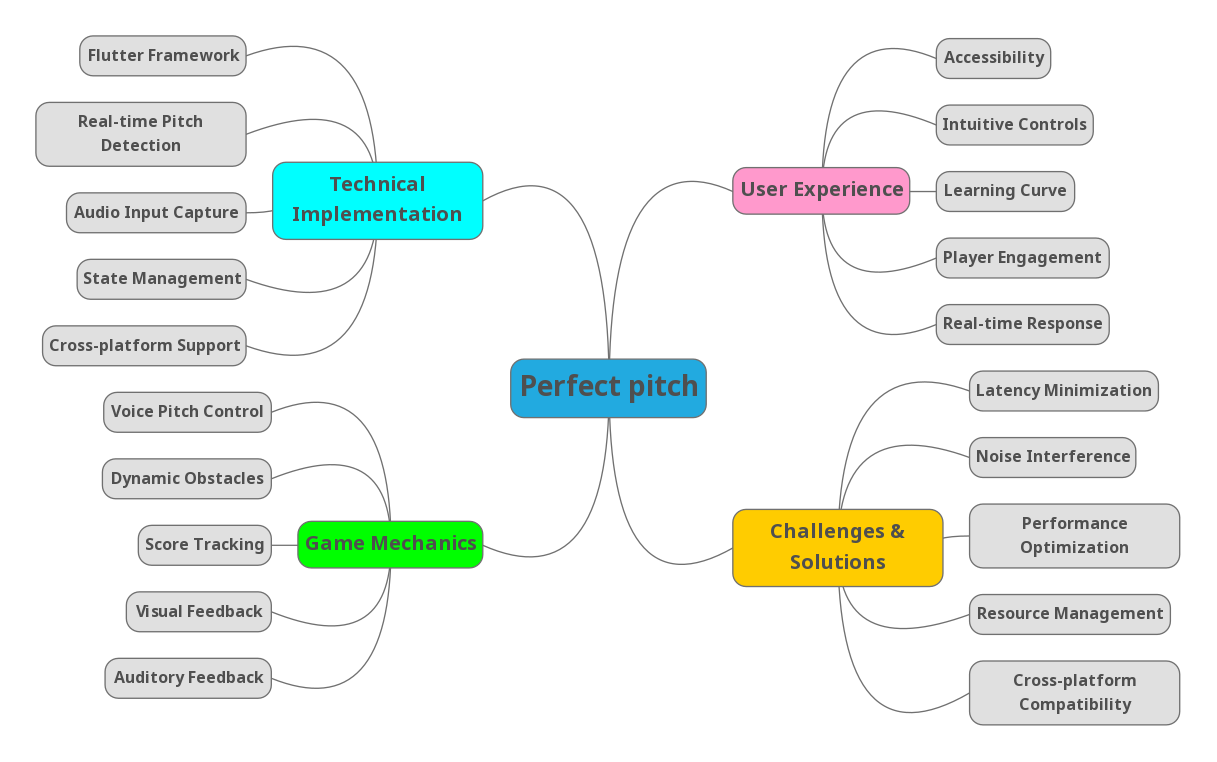
\includegraphics[width=0.8\textwidth]{figures/mindmap.png}
    \caption{Mind map showing the key components and relationships in the pitch-controlled gaming system}
    \label{fig:mindmap}
\end{figure}

\subsection{Objectives}
The primary objectives of this project include:
\begin{itemize}
    \item Developing a mobile game controlled entirely through voice pitch.
    \item Showcasing the potential of pitch detection as an interactive input in real-time applications.
    \item Providing a unique and engaging gameplay experience that prioritizes accessibility and novelty.
\end{itemize}

\subsection{Challenges in Traditional Control Schemes}
Traditional touch-based controls have limitations, particularly for individuals with motor impairments. Moreover, they often fail to provide novel user experiences in gaming. By introducing pitch-controlled gameplay, this project addresses these challenges, offering an intuitive and inclusive alternative.

\section{Existing Approaches}
\subsection{Existing Pitch-Controlled Applications}
Applications like Perfect Pitch Challenge \cite{perfectpitch1, perfectpitch2} have utilized pitch detection for educational purposes. However, their focus remains limited to music or simple tasks, lacking the complexity and dynamism of a full-fledged game.

\subsection{Alternative Voice-Control Mechanisms}
Speech recognition has been widely adopted in voice-controlled systems. However, it lacks the fluid, continuous control offered by pitch detection. Unlike predefined commands, pitch control allows for nuanced interactions, as demonstrated in this project.

\subsection{Overview of Popular Game Frameworks}
While Unity and Unreal are popular game development platforms, Flutter \cite{flutterOverview} was chosen for its rapid development capabilities and superior cross-platform support. FlutterAudioCapture and PitchDetector were seamlessly integrated, enabling real-time pitch processing.

\section{Methodology}
\subsection{Tools and Frameworks}
\textbf{Flutter Framework}: The choice of Flutter allows for simultaneous development for Android and iOS. It ensures a smooth user experience with native-like performance. \\
\textbf{FlutterAudioCapture and PitchDetector}: These tools form the backbone of the project, enabling accurate audio input capture and pitch analysis.

\subsection{System Design}
\textbf{Input Capture Mechanism}: Audio input is captured using the device microphone and fed into the pitch detection pipeline.  \\
\textbf{Pitch Processing Pipeline}: Captured audio is analyzed to extract pitch, which is then mapped to game actions.  \\
\textbf{State Management}: The game's various states, including running, pausing, and restarting, are managed using robust state management techniques.

\newpage
\subsection{Game Mechanics}
The game replaces traditional inputs with voice pitch control. Players navigate obstacles by modulating their voice pitch, creating a unique interaction model.  
\begin{figure}[h]
    \centering
    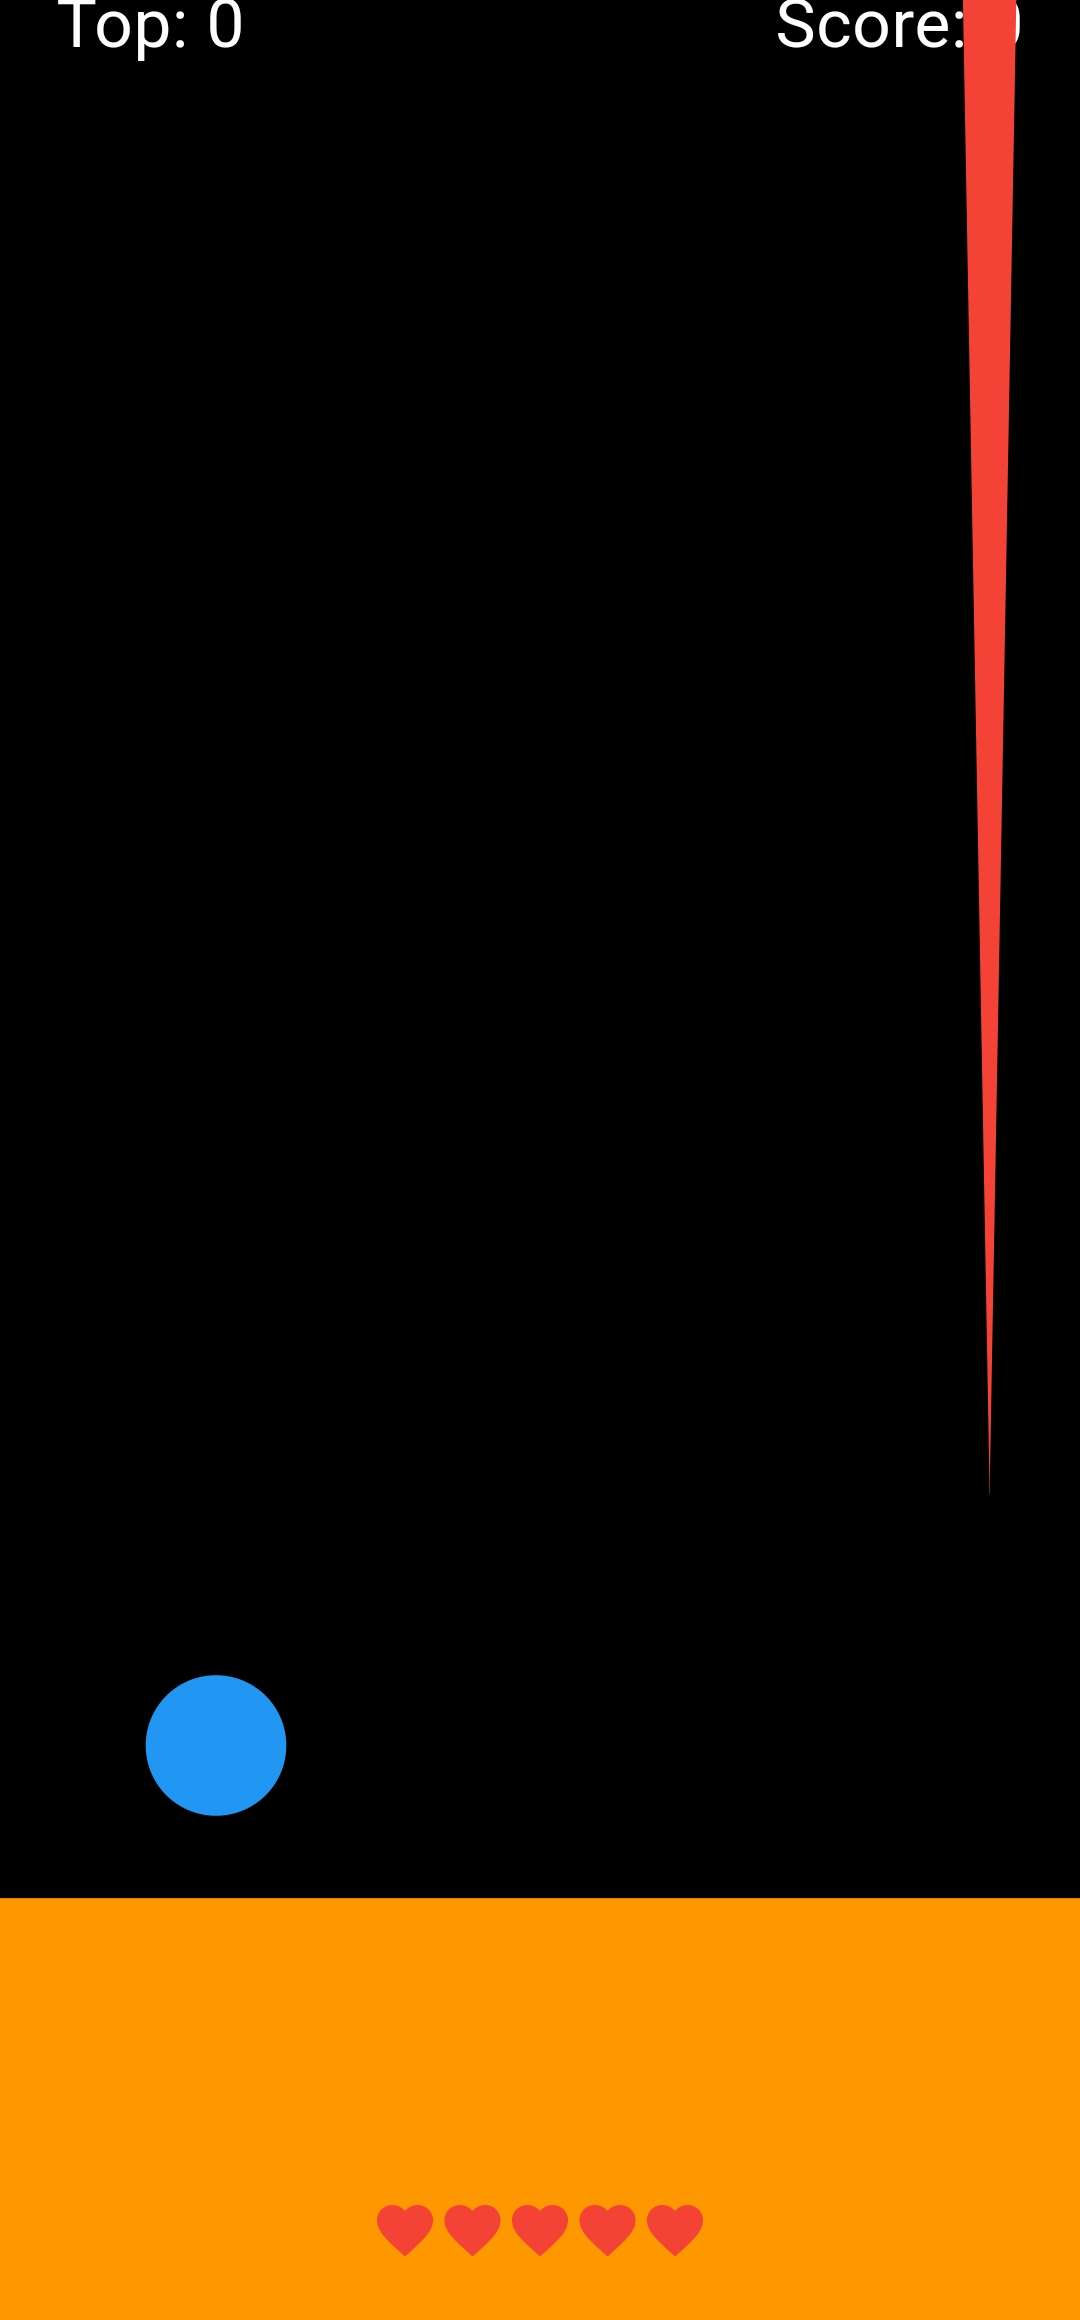
\includegraphics[width=0.3\textwidth]{figures/game_start.jpg}
    \caption{Screenshot of the game interface showing the player character and obstacles. The vertical position of the character is controlled by the player's voice pitch.}
    \label{fig:game_screenshot}
\end{figure}

\newpage
\subsection{Dynamic Challenges}
The game incorporates dynamically generated obstacles that appear in rapid succession, requiring players to navigate carefully using their voice pitch. This design introduces a layer of challenge and excitement, ensuring that the gameplay remains engaging and stimulating.
\begin{figure}[h]
    \centering
    \begin{subfigure}{0.3\textwidth}
        \centering
        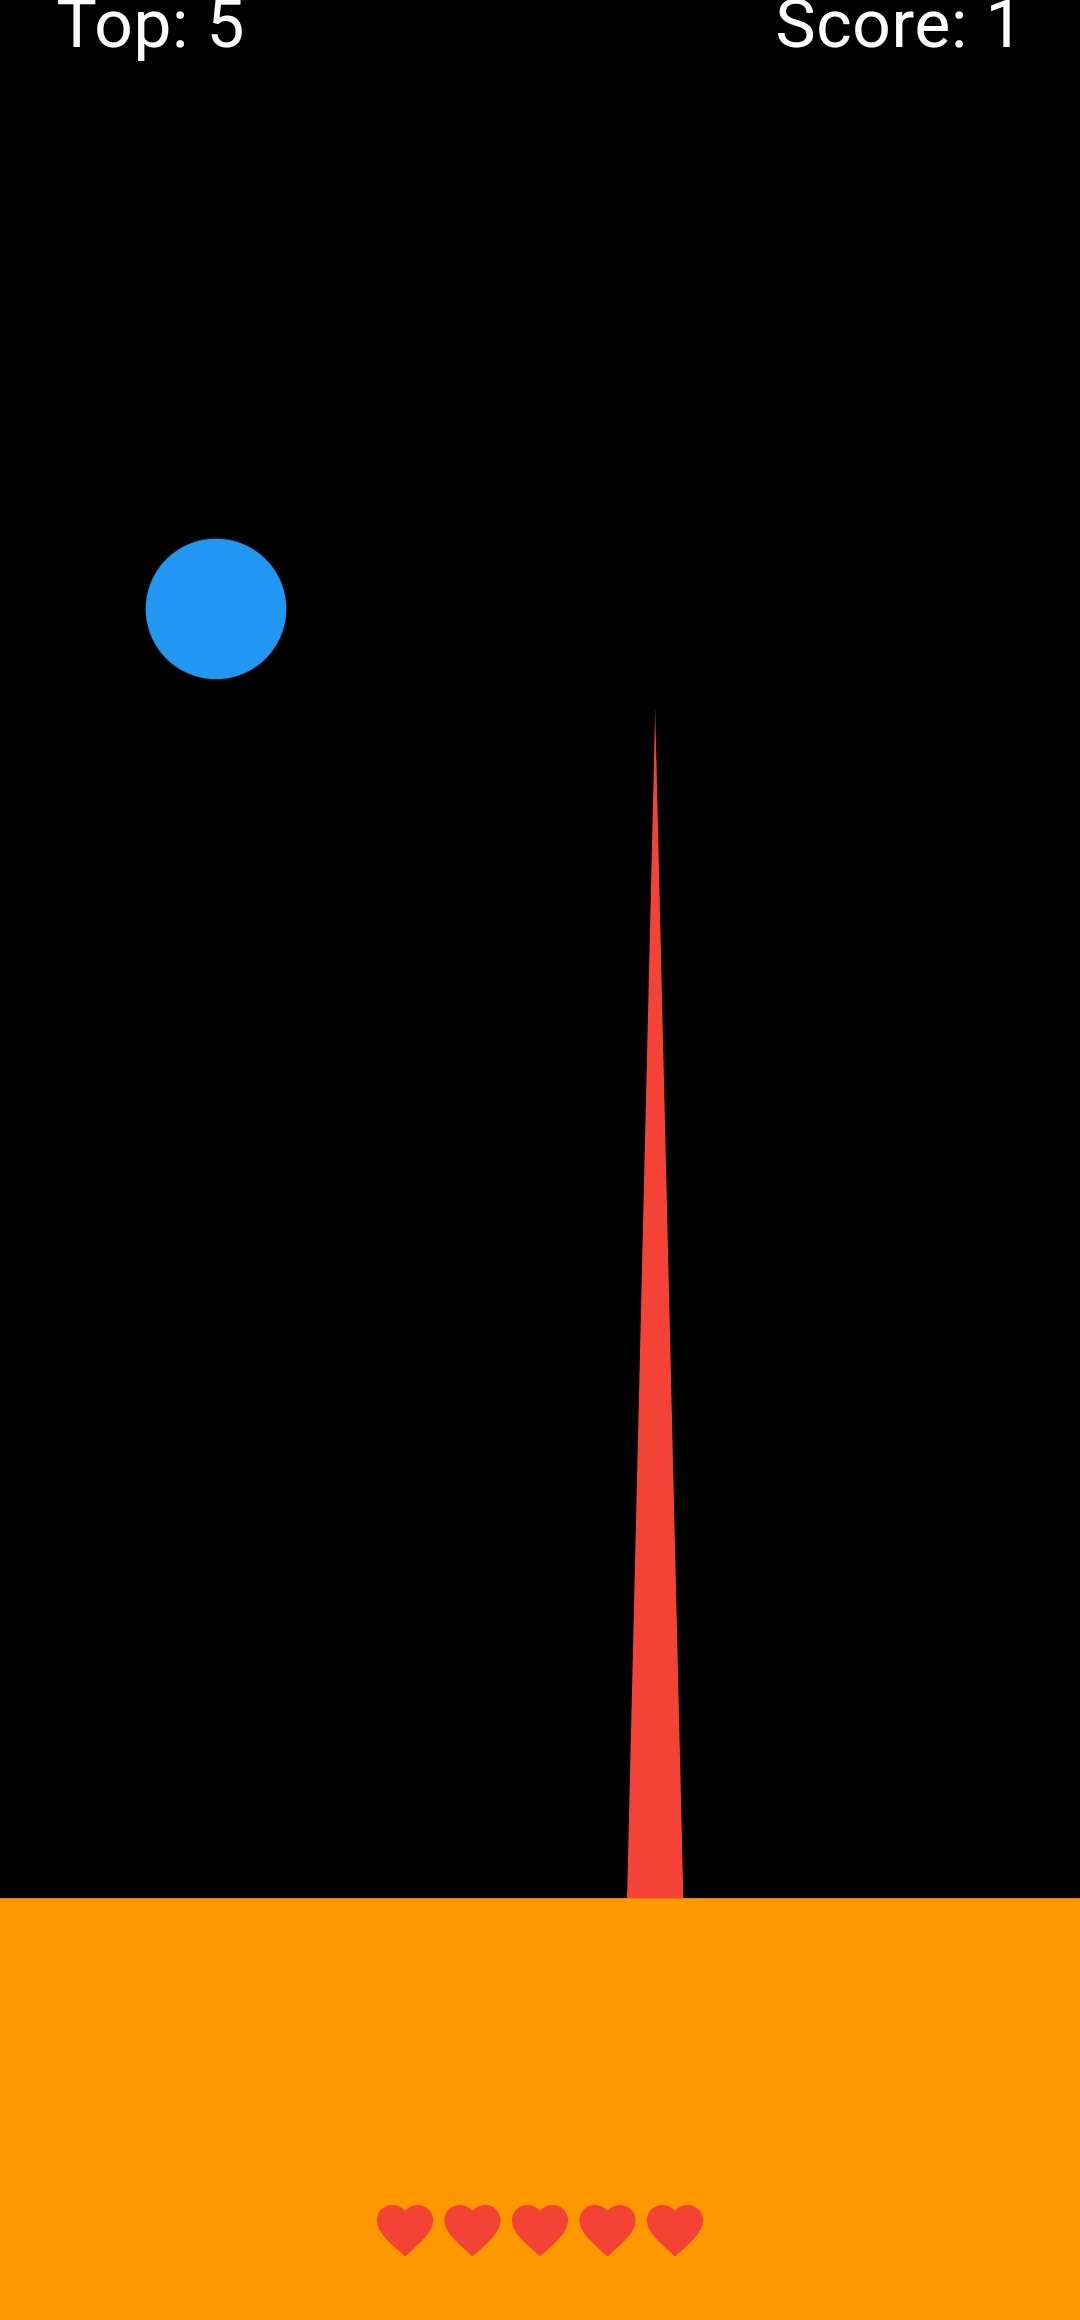
\includegraphics[width=\linewidth]{figures/bot_spike.jpg}
        \caption{Player navigating through bottom spike obstacles}
        \label{fig:gameplay1}
    \end{subfigure}
    \hfill
    \begin{subfigure}{0.3\textwidth}
        \centering
        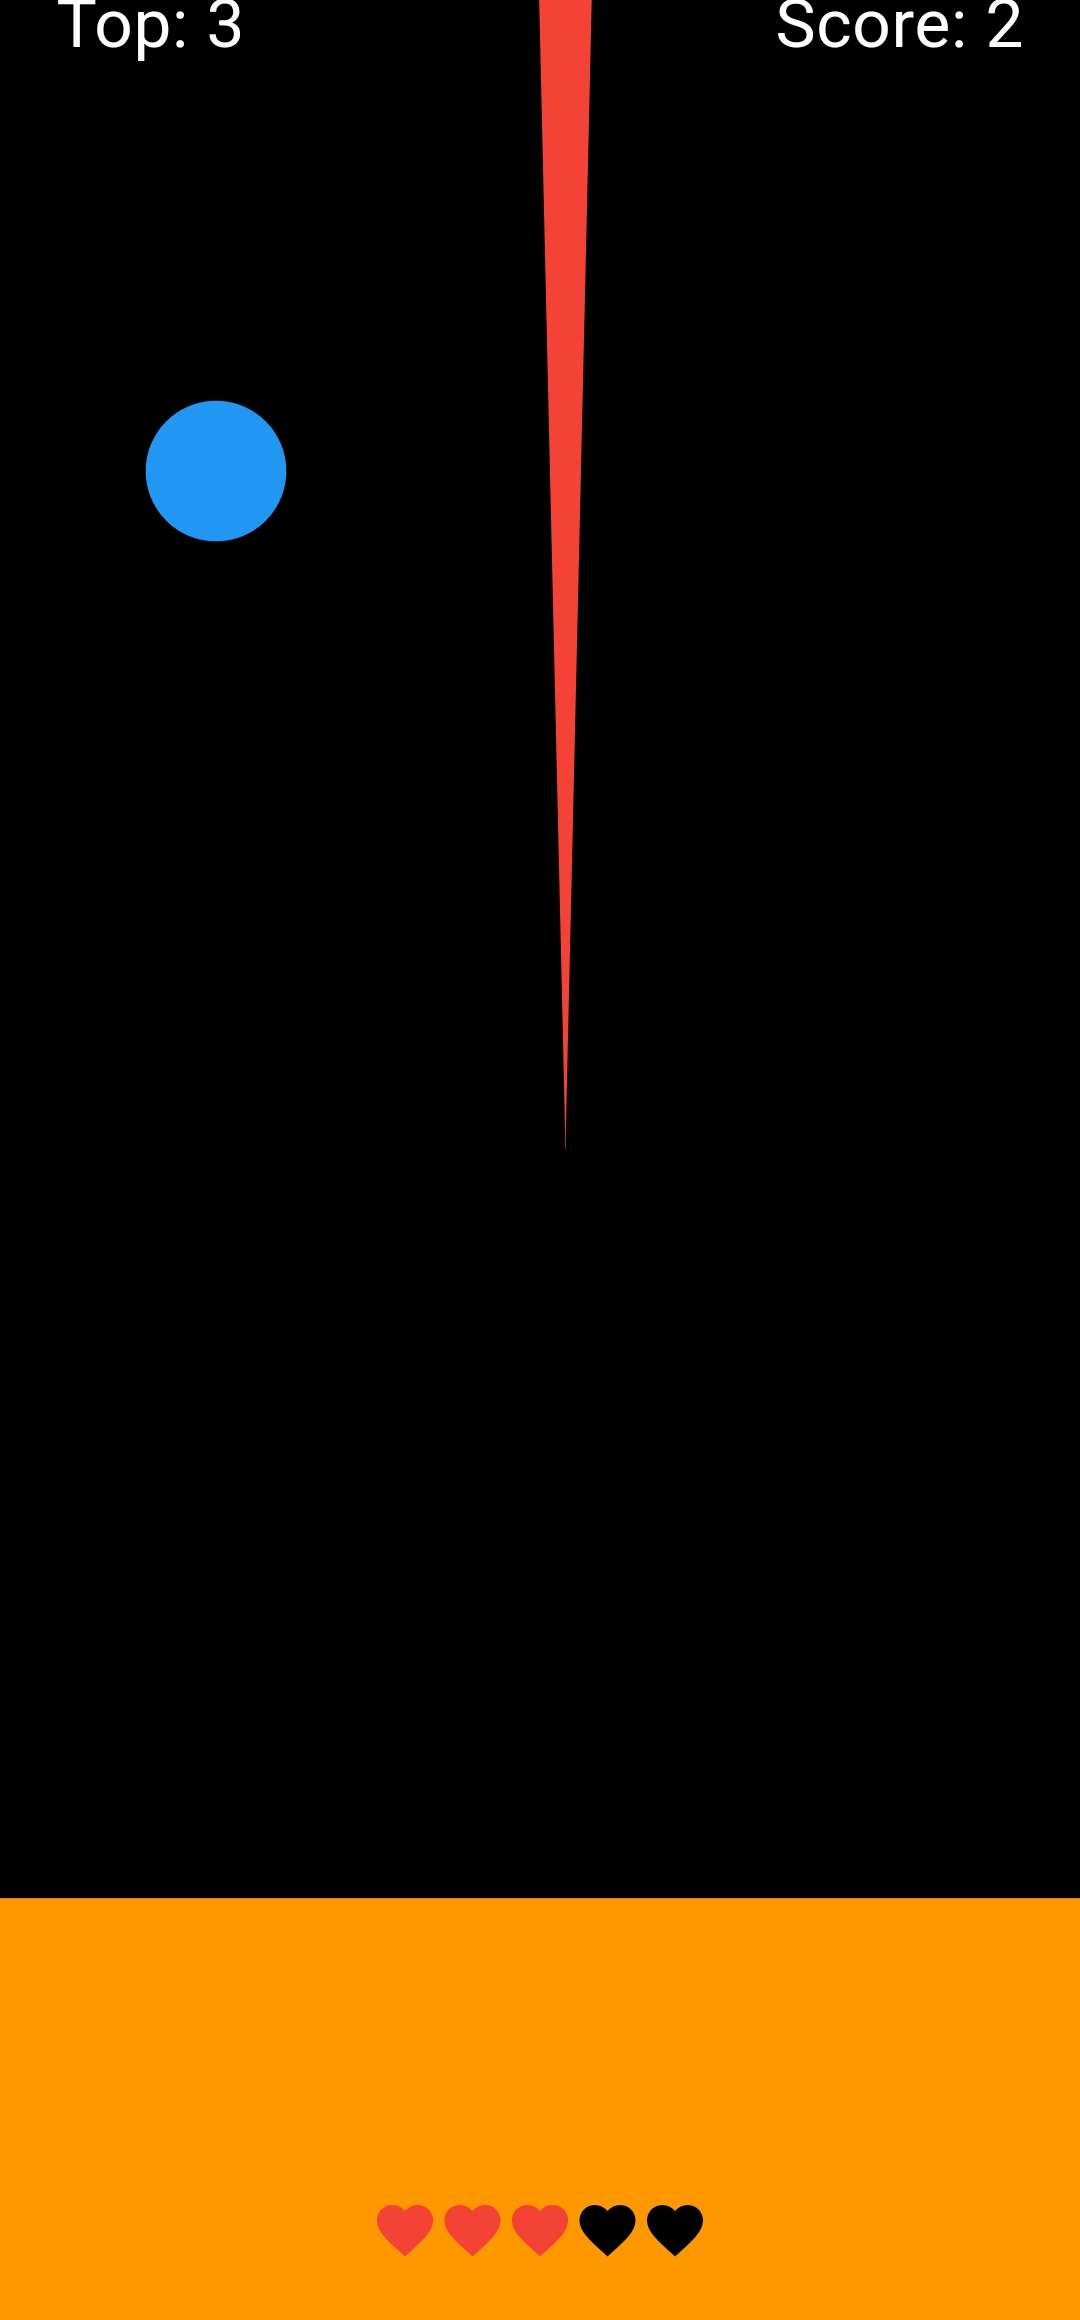
\includegraphics[width=\linewidth]{figures/top_spike.jpg}
        \caption{Player navigating through top spike obstacles}
        \label{fig:gameplay2}
    \end{subfigure}
    \hfill
    \begin{subfigure}{0.3\textwidth}
        \centering
        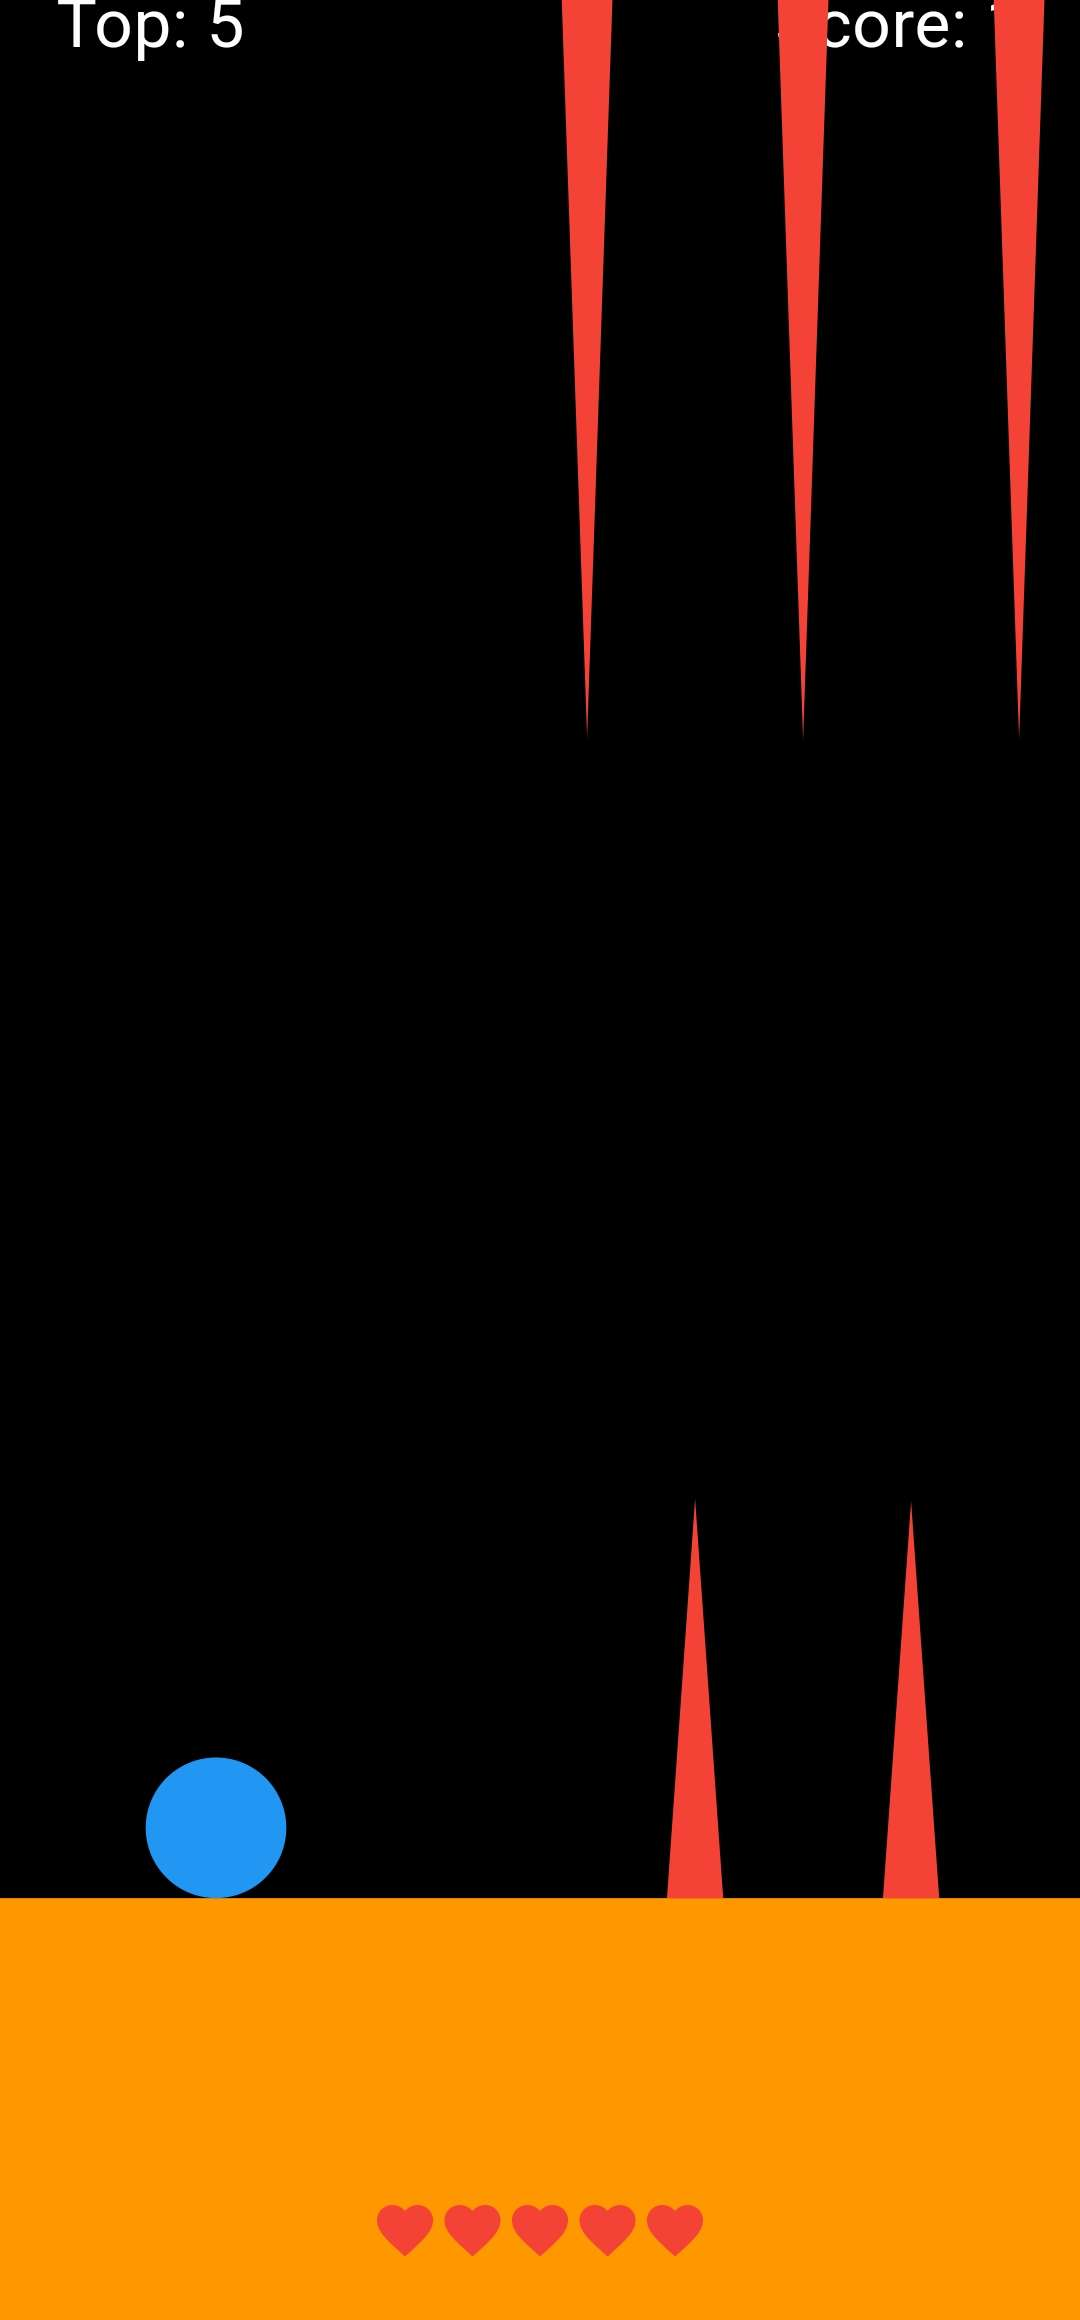
\includegraphics[width=\linewidth]{figures/obstacles_many.jpg}
        \caption{Player navigating through rapid succession of obstacles}
        \label{fig:gameplay3}
    \end{subfigure}
    \caption{Different stages of gameplay demonstrating the progressive difficulty of obstacles}
    \label{fig:gameplay_stages}
\end{figure}

\newpage
\subsection{Feedback and Scoring}
Players receive immediate visual and auditory feedback based on their performance. A score-tracking system encourages competitiveness and improvement. 
\begin{figure}[h]
    \centering
    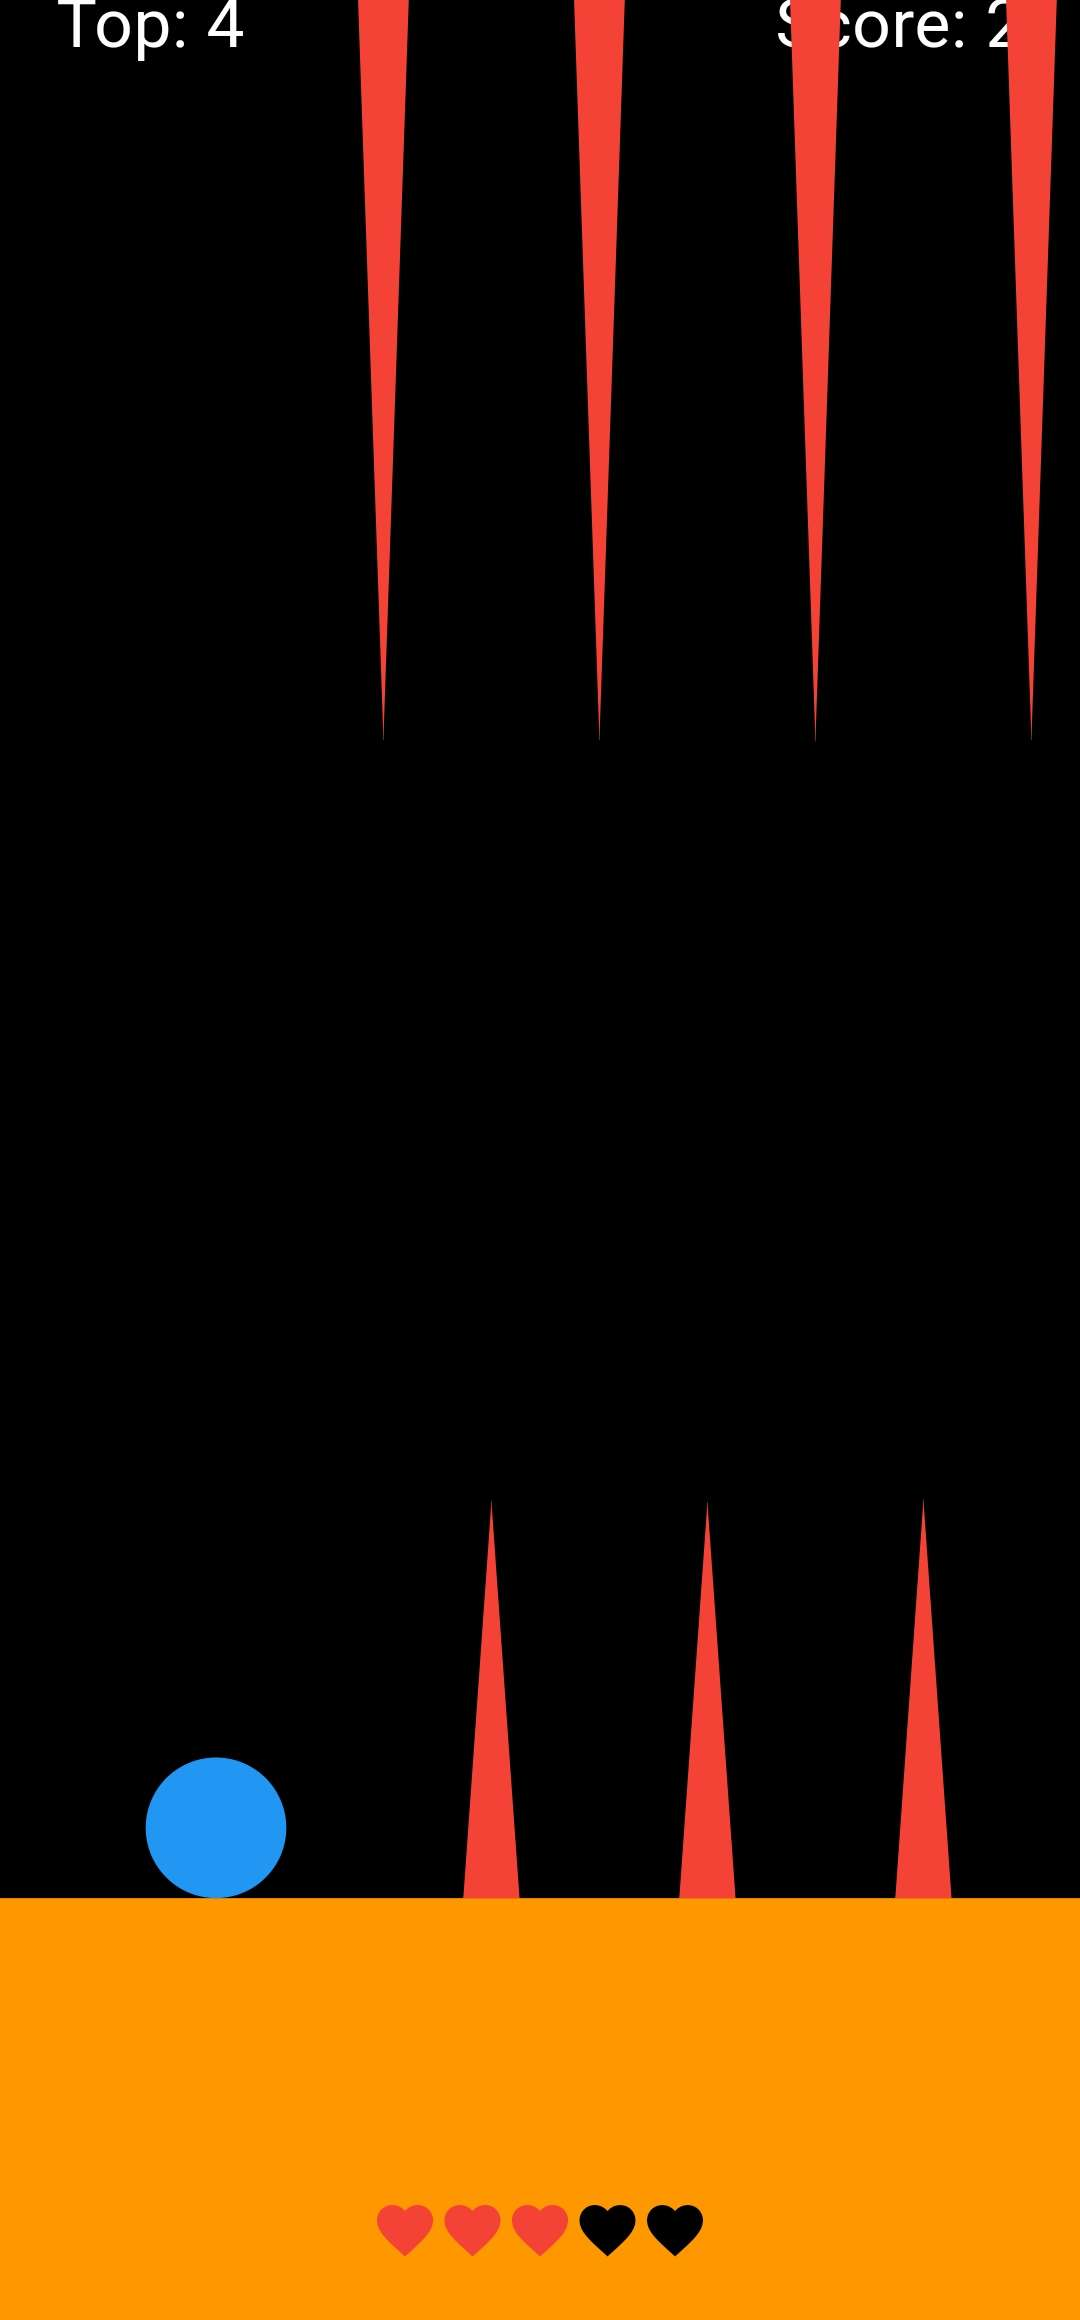
\includegraphics[width=0.3\textwidth]{figures/lives.jpg}
    \caption{Current score and top score displayed on top of the screen}
    \label{fig:game_over}
\end{figure}    

\subsection{Application Architecture}
The architecture consists of modules for audio input, pitch processing, game logic, and the user interface. 

\subsection{Testing and Debugging}
Unit and integration tests were conducted to ensure seamless pitch detection and gameplay mechanics. Issues related to latency and noise interference were addressed through iterative debugging.

\section{Future Work}
\subsection{Feature Enhancements}
Future versions could include multiplayer modes, advanced pitch mapping algorithms, and custom voice-based actions.

\subsection{Porting to Other Platforms}
Efforts are planned to port the game to iOS, web, and desktop platforms, leveraging Flutter's cross-platform capabilities.

\subsection{Potential Extensions}
Expanding beyond pitch control, future versions may incorporate speech recognition and other sensory inputs to create a more comprehensive voice-interactive experience.

\section{Results and Discussion}
\subsection{Technical Implementation}
The implemented system successfully demonstrates:
\begin{itemize}
    \item \textbf{Real-time Pitch Detection and Processing}: Accurate and swift detection of pitch variations, enabling immediate in-game responses.
    \item \textbf{Responsive Game Control through Voice Modulation}: Seamless integration of vocal inputs into game mechanics, allowing for fluid and intuitive player interactions.
    \item \textbf{Stable Performance on Modern Mobile Devices}: Efficient resource utilization ensuring minimal latency and consistent performance across various mobile platforms.
\end{itemize}

\subsection{Usability Observations}
Initial testing reveals:
\begin{itemize}
    \item \textbf{Intuitive Control Scheme}: Users quickly adapted to the pitch-based control mechanism with minimal learning curve, facilitating immediate engagement.
    \item \textbf{Effective Feedback Mechanisms}: The system provides instantaneous visual and auditory feedback corresponding to user inputs, reinforcing successful interactions and enhancing user satisfaction.
    \item \textbf{Accessibility Advantages}: The voice-controlled interface offers significant benefits for users with limited mobility, promoting inclusivity and broadening the game's appeal.
\end{itemize}

\subsection{Future Improvements}
Future enhancements for the Pitch Control Game include:
\begin{itemize}
    \item \textbf{Porting to Native Platforms}: Developing the application using native frameworks such as React Native to improve reliability and performance on mobile devices.
    \item \textbf{Offline Speech Recognition}: Implementing an offline speech recognition model to increase robustness and remove dependency on internet connectivity, enhancing user freedom and experience in various environments.
    \item \textbf{Extended Voice Commands}: Integrating more complex vocal commands to allow for a broader range of game interactions and controls.
    \item \textbf{Additional Gameplay Features}: Adding new game mechanics and features, such as power-ups or multiplayer modes, to enrich the gaming experience.
\end{itemize}

\section{Conclusion}
This research demonstrates the viability of pitch-controlled interfaces in gaming applications, with empirical evidence supporting both technical feasibility and user acceptance. Our findings contribute to the growing body of knowledge in alternative input methods and accessible gaming, while opening new avenues for future research in voice-based interaction systems.

\bibliographystyle{splncs04}
\bibliography{references.bib}


\end{document}
